%/*******************************************************************************
% * Copyright (c) 2007, G. Weirich
% * All rights reserved. This program may not be distributed
% * or modified without prior written consent
% *
% * Contributors:
% *    G. Weirich - initial implementation
% *
% *  $Id: anleitung.tex 231 2007-08-23 19:12:43Z Gerry $
% *******************************************************************************/

\documentclass[a4paper]{scrartcl}
\usepackage{german}
\usepackage[utf8]{inputenc}
\usepackage{makeidx}
\usepackage[pdftex]{graphicx}
\DeclareGraphicsExtensions{.pdf,.jpg,.png}
\makeindex
\usepackage{floatflt}
\usepackage[]{hyperref}
\usepackage{color}
\title{Elexis-Medikamente-BAG}
\author{Gerry Weirich}

\begin{document}
\maketitle
\section{Einführung}

Dies ist ein Medikamente-Plugin, das als Datenbasis die vom BAG veröffentlichte Excel\texttrademark-Version der Spezialitätenliste verwendet. Darüberhinaus hat es einige funktionelle Erweiterungen gegenüber dem älteren, Galdat-basierten Plugin.

\section{Voraussetzungen}
Dieses Plugin benötigt Elexis 1.1.1 oder höher.

\medskip

Dieses Plugin kann entweder allein oder auch zusammen mit dem existierenden Galdat-Plugin verwendet werden. In letzterem Fall wird auch eine gemeinsame Datenbasis verwendet. Das heisst, bei Medikamenten der SL werden die zusätzlichen SL-spezifischen Angaben integriert, die nicht-SL-Artikel bleiben weiterhin vorhanden, aber haben weiterhin nur die Galdat-Informationen. (Die Zusätzlichen Informationen der SL-Medikamente sind im Wesentlichen Inhaltsstoffe, therapeutische Gruppe und Generika-Status)

\section{Verwendung}

%\begin{figure}
    %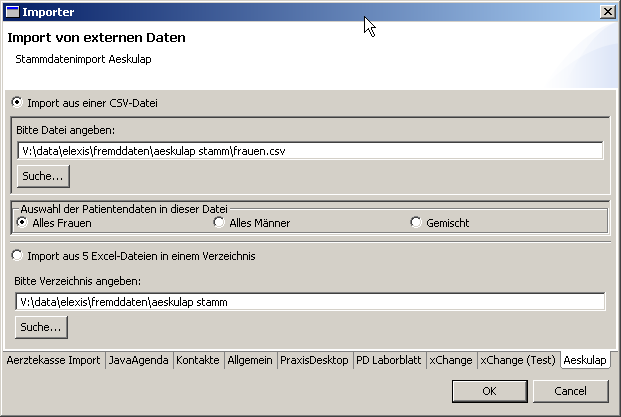
\includegraphics[width=0.8\textwidth]{aeskulap}
    %\caption{Aeskulap-Import}
    %\label{fig:aeskulap}
%\end{figure}

In der Listenauswahl haben Sie jetzt einen Generika-Filterknopf und drei verschiedene Felder zur Auswahl:
\begin{itemize}
    \item Name: Medikamente nach Name filtern
    \item Inhalt: Medikamente nach Inhaltsstoff filtern
    \item Notiz: Medikamente nach eigenen Notizen filtern. 
\end{itemize}
Wenn der Generika-Knopf eingerastet ist, werden bei allen \textit{nachfolgenden} Filterungen nur Generika angezeigt.

\medskip

Wenn Sie auf ein Medikament mit der rechten Maustaste klicken, erhalten Sie ausserdem die Option "'selbe therap. Gruppe"'. Auswahl dieser Option bewirkt, dass alle Medikamente, die zur selben therapeutischen Gruppe gehören, angezeigt werden.

\end{document} 